\begin{figure}[t]
    \centering
    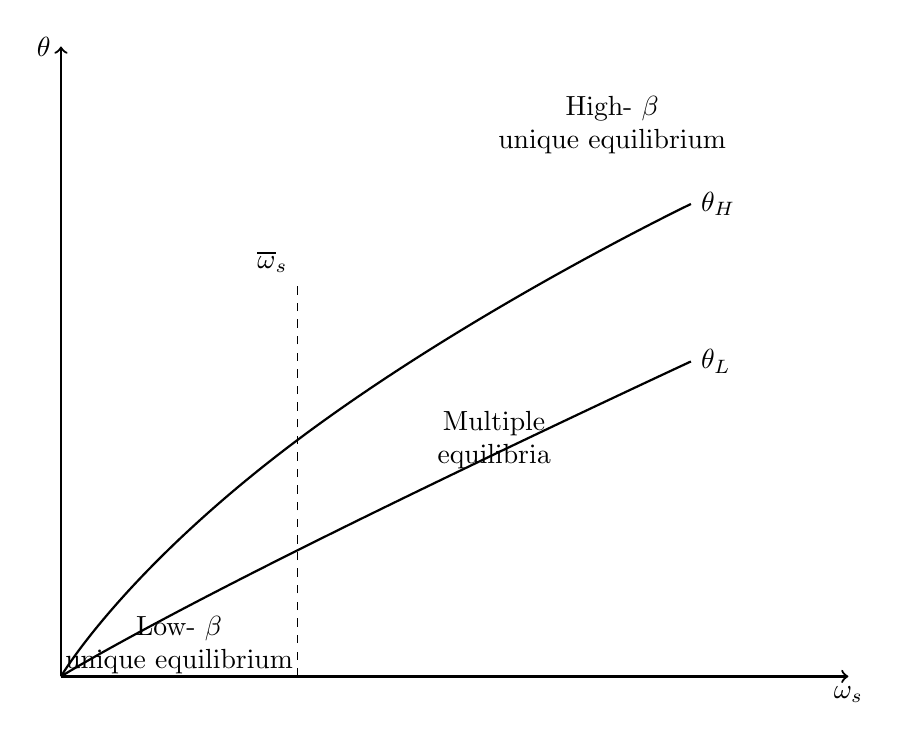
\begin{tikzpicture}[scale=2.0]

    % Axes
\draw[->, thick] (0,0) -- (5,0) node[below] {$\omega_s$};
\draw[->, thick] (0,0) -- (0,4) node[left] {$\theta$};

% Curves
\draw[thick] plot[smooth, tension=1] coordinates {(0,0) (1.5,1.5) (4,3)} node[right] {$\theta_H$};
\draw[thick] plot[smooth, tension=1] coordinates {(0,0) (1.5,0.8) (4,2)} node[right] {$\theta_L$};

% Dotted line for critical point
\draw[dashed] (1.5,0) -- (1.5,2.5) node[above left] {$\overline{\omega}_s$};

% Labels for regions
\node at (0.75,0.2) [align=center] {Low- $\beta$ \\ unique equilibrium};
\node at (2.75,1.5) [align=center] {Multiple \\ equilibria};
\node at (3.5,3.5) [align=center] {High- $\beta$ \\ unique equilibrium};
    
    % Fill by gray
    %\fill[gray!20] 
        %(0.4,0.5+0.2) to [out = 55, in = 190, looseness=1.0](3,1.8+0.2)
        %-- (3,0.64+0.2)
       % to [out = 5, in = 182, looseness=0.5] (0.4,0.5+0.2)
       % -- cycle;

    % Fill below theta_L and right of threshold with dots
    %\fill[pattern=dots, pattern color = black!25] 
       % (0.4,0.5+0.2) to [out = 5, in = 182, looseness=0.5](3,0.64+0.2)
       % -- (3, 0)
       % to (0.4,0)
       % -- cycle;
        
    % Labels
    %\node at (0.8+0.1,1.2+0.65) {\footnotesize High-$\beta$ equilibrium};
    %\node at (2,0.95+0.2) {\footnotesize Multiple equilibria};
    %\node at (1.6,0.3+.1) {\footnotesize Low-$\beta$ equilibrium};
    

    % Points at the end of curves
   % \node[right] at (3,1.8+0.2) {$\theta_H$};
    %\node[right] at (3,0.8) {$\theta_L$};

    % Threshold for multiple eqm
   % \draw[thick] (0.4,0.5+0.2) -- (0.4,0.0) node[below] {$\tilde{\omega}_{s}$};

    \end{tikzpicture}
    \caption{Equilibrium Characterization with Exogenous $\theta$}
    \caption*{\footnotesize{Note: This figure illustrates the equilibrium states using the reputation concern, $\theta$, and the skill potential, $\omega_{s}$.}}
    \label{fig:theta}
\end{figure}